\documentclass[12pt]{exam}
\usepackage[top=1in, bottom=1in, left=.45in, right=.45in]{geometry}
\usepackage{amsmath,amsthm,amssymb,amstext}
\usepackage{enumerate,enumitem}
\usepackage{tikz,float,graphicx}
\usepackage{microtype}
\usepackage{bm,tikz}
    \usetikzlibrary{calc}
\usepackage{multicol}
\usepackage{nicematrix}
\usepackage[framemethod=tikz]{mdframed}

\newcommand{\course}{MTH 234 Summer 2021}
\newcommand{\qdate}{The Cross Product} %PUT DATE HERE
\newcommand{\quiz}{Group Work} 

\newcommand{\ba}{\bm{a}}
\newcommand{\bb}{\bm{b}}
\newcommand{\bc}{\bm{c}}
\newcommand{\bi}{\bm{i}}
\newcommand{\bj}{\bm{j}}
\newcommand{\bk}{\bm{k}}
\newcommand{\gen}[1]{\left\langle #1 \right\rangle}

\newtheorem*{definition}{Definition}
\surroundwithmdframed[]{definition}
\newtheorem*{remark}{Remark}
\surroundwithmdframed[]{remark}
\newtheorem*{theorem}{Theorem}
\surroundwithmdframed[]{theorem}

%%%%%%%%%%%%%%%%%%%%%%%
% HEADER AND FOOTER
%%%%%%%%%%%%%%%%%%%%%%%
\pagestyle{headandfoot}
\firstpageheadrule
\runningheadrule
\firstpageheader{\course}{\quiz}{\qdate}
\runningheader{\course}{\quiz}{\qdate}
\runningfooter{}{}{}


\usepackage{color}
\shadedsolutions
\definecolor{SolutionColor}{rgb}{0.8,0.9,1}
\printanswers
%\noprintanswers


\begin{document}
\section*{Properties and Applications of the Cross Product}
\begin{remark}
    For convenience, if \(\ba=\gen{a_1,a_2,a_3}\) and \(\bb=\gen{b_1,b_2,b_3}\),
    \begin{align*}
        \ba\times\bb & = \left|
            \begin{NiceMatrix}
                \bi & \bj & \bk \\
                a_1 & a_2 & a_3\\
                b_1 & b_2 & b_3
            \end{NiceMatrix}
        \right|\\
        = \bi
        \left|\begin{NiceMatrix}
             a_2 & a_3\\
             b_2 & b_3
        \end{NiceMatrix}\right|
            -\bj
        \left|\begin{NiceMatrix}
            {a_1} &  a_3\\
            {b_1} &  b_3
        \end{NiceMatrix}\right|
        +\bk
        \left|\begin{NiceMatrix}
            {a_1} & {a_2}  \\
            {b_1} & {b_2} 
        \end{NiceMatrix}\right|
        \\
        & = (a_2b_3-b_2a_3)\bi-(a_1b_3-b_1a_3)\bj+(a_2b_3-b_2a_3)\bk
    \end{align*}
\end{remark}
\begin{theorem}
    Let \(\ba,\bb,\bc\) be vectors and let \(r,s\) be scalars.
    \begin{multicols}{2}
        \begin{enumerate}[label={\alph*.}]
            \item \(\ba\times \bb = -\bb\times \ba\)
            \item \((r\ba) \times (s\bb) = (rs)(\ba\times\bb)\)
            \item \(\bm{0}\times\ba=\bm{0}\)
            \item \(\ba\times(\bb+\bc) = \ba\times\bb+\ba\times\bc\)
            \item \((\bb+\bc)\times\ba = \bb\times\ba+\bc\times\ba\)
        \end{enumerate} 
    \end{multicols}
\end{theorem}

\begin{questions}

\question Let \(\ba=\gen{1,1,-1}\) and \(\bb=\gen{-2,-4,-6}\).
\begin{parts}
    \part Compute \(\ba\times\bb\).
    \ifprintanswers
        \begin{solution}
            \begin{align*}
                \ba\times\bb & = 
                    \left|
                        \begin{NiceMatrix}
                            \bi & \bj & \bk \\
                            1 & 1 & -1\\
                            -2 & -4 & -6\\
                        \end{NiceMatrix}
                    \right|\\
                    & = (-6-4)\bi-(-6-2)\bj+(-4-(-2))\bk\\
                    & = -10\bi+8\bj-2\bk\\
                    & = \gen{-10,8,-2}
            \end{align*}
        \end{solution}
    \else
        \vfill
    \fi

\noindent Use your result and the properties above to compute the following:

\phantom{.}

    \part \(\bb\times\ba\)
    \ifprintanswers
        \begin{solution}
            \[
                \bb\times\ba = -\ba\times \bb = \gen{10,-8,2}
            \]
        \end{solution}
    \else
        \vfill
    \fi    

    \part \(\gen{4,4,-4}\times\gen{2,4,6}\) (hint: try to express each vector as a scalar times \(\ba\) or \(\bb\))
    \ifprintanswers
        \begin{solution}
            \[
                \gen{4,4,-4}\times\gen{2,4,6} = (4\ba)\times(-\bb) = -4(\ba\times\bb) = \gen{40,-32,8}
            \]
        \end{solution}
    \else
        \vfill
    \fi    

    \part \(\ba\times(\bb+\bb)\)
    \ifprintanswers
        \begin{solution}
            \[
                \ba\times(\bb+\bb) = \ba\times(2\bb)=2(\ba\times\bb)= \gen{-20,16,-4}
            \]
        \end{solution}
    \else
        \vfill
    \fi    

    \part \(\ba\times(\bb+\bc)+(\bb+\bc)\times\ba\) where \(\bc\) is any vector.
    \ifprintanswers
        \begin{solution}
             Since \((\bb+\bc)\times\ba= -\ba\times(\bb+\bc)\), the answer is \(\bm{0}\).
        \end{solution}
    \else
        \vfill
    \fi    
\end{parts}

\ifprintanswers

    \newpage
\fi




\begin{remark}
    Recall that a parallelogram with side lengths \(x\) and \(y\) has area
        \[
            A(x,y) = xy\sin\theta
        \]
    If we represent the sides of a parallelogram as vectors, we can rewrite this as the following
\end{remark}

\begin{theorem}
        The area of a parallelogram formed by vectors \(\ba\) and \(\bb\) if given by
        the magnitude of their crossproduct, i.e.
        \[
            A = |\ba||\bb|\sin\theta = |\ba\times\bb|
        \]

\begin{center}
        \begin{tikzpicture}
            \draw[->] (0,0)--(3,0) node[midway,below] {$\ba$};
            \draw[->] (0,0)--(2,2) node[midway,above] {$\bb$};
            \draw[dashed] (2,2)--(5,2);
            \draw[dashed] (3,0)--(5,2);
            \draw (1,0) arc (0:45:1) node[midway,right] {$\theta$};
        \end{tikzpicture}
\end{center}
\end{theorem}

\question Find the area of the paralellogram with sides represented by
    \[
        \ba=\gen{2,-2,0} ~~~\text{and}~~~ \bb=\gen{0,3,2}
    \]
    \ifprintanswers
        \begin{solution}
            First we will find the crossproduct
            \[
                \ba\times\bb = 
                    \left|\begin{NiceMatrix}
                        \bi & \bj & \bk\\
                        2 & -2 & 0\\
                        0 & 3 & 2
                        \end{NiceMatrix}\right| = \gen{-4,-4,6}
            \]
            Then the area is 
            \[
                |\gen{-4,-4,6}|=\sqrt{16+16+36}=2\sqrt{17}~\text{units}^2
            \]
        \end{solution}
    \else
        \vfill
    \fi    



\question Find the area of the triangle with vertices 
\[
    P(0,0,-3),\quad Q(4,2,0),\quad \text{and}~~R(3,3,1).
\]

\ifprintanswers
        \begin{solution}
            We first find vectors \(PQ\) and \(PR\).
            \begin{align*}
                PQ & = \gen{4,2,0}-\gen{0,0,-3}=\gen{4,2,3}\\
                PR & = \gen{3,3,1}-\gen{0,0,-3}=\gen{3,3,4}
            \end{align*}
        Then the area of the \textbf{paralellogram} with sides \(PQ\) and \(PR\) is
        \[
            |PQ\times PR| = |\gen{-1,-7,6}| = \sqrt{86}~\text{units}^2.
        \]
        And the area of the triangle is 
        \[
            \frac{1}{2}(\text{area of the paralellogram})=\frac{1}{2}\sqrt{86}.
        \]
        
        \end{solution}
    \else
        \vfill
    \fi    

\newpage

\begin{remark}
    Recall that \(\ba\times\bb\) is orthogonal to both \(\ba\) and \(\bb\)
\end{remark}

\question Find two unit vectors orthogonal to \(\bm{j}-\bm{k}\) and \(\bm{i}+\bm{j}\).
\ifprintanswers
        \begin{solution}
            We will first find the crossproduct
            \[
            \gen{0,1,-1}\times\gen{1,1,0} = \gen{1,-1,-1}
            \]
            This is a vector orthogonal to both of the given vectors. Then a unit vector is
            \[
                \frac{1}{|\gen{1,-1,-1}}\gen{1,-1,-1}=\gen{\frac{1}{\sqrt{3}},\frac{1}{\sqrt{3}},-\frac{1}{\sqrt{3}}}.
            \]
            Multiplying this result by \(-1\) gives a vector in the opposite direction with the same magnitude, so a second distinct unit vector is
            \[
                \gen{-\frac{1}{\sqrt{3}},\frac{1}{\sqrt{3}},\frac{1}{\sqrt{3}}}
            \]
        \end{solution}
    \else
        \vfill
    \fi    

\question Let \(\ba=\gen{-2,10,0}\) and \(\bb=\gen{7,7,7}\). Compute \((\ba\times\bb)\cdot (\bm{i}+\bm{k})\).

\ifprintanswers
        \begin{solution}
            \[
                \gen{-2,10,0}\times\gen{7,7,7}=\gen{70,14,-84}.
            \]
            Then 
            \[
              (\gen{-2,10,0}\times\gen{7,7,7})\cdot\gen{1,0,1}=70-84=-14.
            \]
        \end{solution}
    \else
        \vfill
    \fi    

\question Let \(\ba,\bb,\bc\) be vectors. Determine if the following are true or false. If false, give an example showing why the statement is false or explain your thinking.
\begin{parts}
    \part \(2(\ba\times\bb) = (2\ba)\times(2\bb)\)
        \begin{choices}
            \choice True \CorrectChoice False
        \end{choices}
        \begin{solution}
            See property (b) of the Theorem on page 1.
        \end{solution}

    \part \((2\ba)\times\bb = \ba\times(2\bb)\)
        \begin{choices}
            \CorrectChoice True \choice False
        \end{choices}

    \part \(|\ba\times\bb|=|\bb\times\ba|\)
        \begin{choices}
            \CorrectChoice True \choice False
        \end{choices}
    \part \(|(-2\ba)\times(\pi\bb)|=-2\pi|\ba\times\bb|\)
        \begin{choices}
            \choice True \CorrectChoice False
            \begin{solution}
                \[
                    |(-2\ba)\times(\pi\bb)| = |-2\pi(\ba\times\bb)| = |-2\pi||\ba\times\bb| = 2\pi|\ba\times\bb|
                \]
            \end{solution}
        \end{choices}
\end{parts}



\question What would you expect \(\mathrm{proj}_{\ba}(\ba\times\bb)\) to be? Draw a picture explaining your thinking.

\ifprintanswers
        \begin{solution}
            Since \(\ba\times\bb\) is orthogonal to \(\ba\), the projection should be a single point, or the 0-vector. See the image below
            \begin{center}
                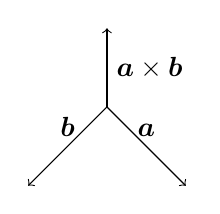
\begin{tikzpicture}
                    \draw[->] (0,0)--(1,-1) node[midway,above] {$\ba$};
                    \draw[->] (0,0)--(-1,-1) node[midway,above] {$\bb$};
                    \draw[->] (0,0)--(0,1) node[midway,right] {$\ba\times\bb$};
                \end{tikzpicture}
            \end{center}
        \end{solution}
    \else
        \vfill
    \fi    

\end{questions}

%%% Orthogonal projection
\end{document}